\documentclass[12pt,a4paper]{article}

\usepackage[utf8]{inputenc}
\usepackage{tikz}
\usetikzlibrary{quotes, angles}
\usepackage[english]{babel} 
\usepackage{biblatex} 
\addbibresource{Bibliography.bib}
\usepackage{graphicx}
\usepackage{tabularx}


\title{MMPS Project 1: Road Construction}
\author{Jack Mortimer, Ruhan Ahmed, Saif-Ullah Hussain,\\ Maya Tetteh, Yuxin Ren\\ Group J}
\date{October 2019}
\begin{document}

\begin{titlepage}
\maketitle
\thispagestyle{empty}
\end{titlepage}

\clearpage
\pagenumbering{arabic}
\textbf{Problem Statement}\\
A road must be constructed between two cities. One of the cities is 40km north and 70km east of the other. The two cities are separated by a strip of forest running from east to west, with a north-south extent of about 7.5km. You are asked to design the most cost-efficient route for the road, taking into 


\begin{tikzpicture}
\draw[gray, thick] (-2,0) -- (9,6);
\filldraw[black] (-2,0) circle (2pt) node[anchor=east] {City A};
\filldraw[black] (9,6) circle (2pt) node[anchor=west] {City B};
\draw[very thick] (-2,3) rectangle (9,4) node[anchor=west]{forest};
\end{tikzpicture}

In the simplest case, the shortest road between the two cities is a straight line through the two points. However, we realised that this is likely not the most cost-efficient route to take as it takes a longer path through the forest than may be necessary. It is clear that the most cost-effective route to take through the forest alone is to travel vertically north. We presumed that this is also unlikely to be the most cost-efficient route as it extends the distance that must be travelled outside of the forest area.\\
\clearpage
\indent Considering these observations we concluded that the most cost-efficient route is to take as direct a path as possible, whilst taking a smaller angle to the normal entering and traveling through the forest. The angle of incidence entering and leaving the forest are the same, as shown. The path taken through the forest is, informally, like a 'kink' in the direct path between the two cities.\\
\indent From this we deduced that it turns out to be irrelevant the exact location of the forest in the north-south direction, and thus its location can be assumed. This is because the angle of incidence entering and leaving the forest being equivalent means that if the forest were moved, the angles remain the same and the total distance is unchanged, the point at which the road enters the forest simply moves east or west and the 'kink' is at a different point along the route from A to B.\\

%Diagram of theorised cheapest route
y\begin{tikzpicture}
\draw[gray, thick] (-2,0) -- (4.5,3);
\draw[gray, thick] (4.5,3) -- (5,4);
\draw[gray, thick] (5,4) -- (9,6);
\filldraw[black] (-2,0) circle (2pt) node[anchor=north] {City A};
\filldraw[black] (9,6) circle (2pt) node[anchor=west] {City B};
\draw[very thick] (-2,3) rectangle (9,4) node[anchor=west]{forest};
\draw [opacity = 0]
(9,6) coordinate (b) node[anchor=west]{}
-- (5,4) coordinate (a) node[anchor=west]{}
-- (5,9) coordinate (c) node[anchor=west]{}
pic["$\theta_{1}$",draw=red,angle eccentricity=1.2,angle radius=1cm, opacity = 1] {angle=b--a--c};
\draw [opacity = 0]
(-2,0) coordinate (b) node[anchor=west]{}
-- (4.5,3) coordinate (a) node[anchor=west]{}
-- (4.5,0) coordinate (c) node[anchor=west]{}
pic["$\theta_{1}$",draw=red,angle eccentricity=1.2,angle radius=1cm, opacity = 1] {angle=b--a--c};
\draw[dashed] (4.5,4) -- (4.5,0);
\draw[dashed] (5,6) -- (5,4);
\draw [opacity = 0]
(4.5,4) coordinate (b) node[anchor=west]{}
-- (4.5,3) coordinate (a) node[anchor=west]{}
-- (5,4) coordinate (c) node[anchor=west]{}
pic["$\theta_{2}$",draw=red,angle eccentricity=1.5,angle radius=0.5cm, opacity = 1]
{angle=c--a--b};
\end{tikzpicture}

\clearpage
For comparison, we calculated the cost in a the case of travelling directly north through the forest, where $\theta_{2}=0^{\circ}$. As the actual price of building the road is unspecified in the problem statement, we let the price per kilometre be 1 arbitrary units outside of the forest and 2 within the forest.

%directly northz
\begin{tikzpicture}
\draw[gray, thick] (-2,0) -- (4,3);
\draw[gray, thick] (4,3) -- (4,4);
\draw[gray, thick] (4,4) -- (9,6);
\filldraw[black] (-2,0) circle (2pt) node[anchor=north] {City A};
\filldraw[black] (9,6) circle (2pt) node[anchor=west] {City B};
\draw[very thick] (-2,3) rectangle (9,4) node[anchor=west]{forest};
\draw [opacity = 0]
(9,6) coordinate (b) node[anchor=west]{}
-- (4,4) coordinate (a) node[anchor=west]{}
-- (4,9) coordinate (c) node[anchor=west]{}
pic["$\theta_{1}$",draw=red,angle eccentricity=1.2,angle radius=1cm, opacity = 1] {angle=b--a--c};
\draw [opacity = 0]
(-2,0) coordinate (b) node[anchor=west]{}
-- (4,3) coordinate (a) node[anchor=west]{}
-- (4,0) coordinate (c) node[anchor=west]{}
pic["$\theta_{1}$",draw=red,angle eccentricity=1.2,angle radius=1cm, opacity = 1] {angle=b--a--c};
\draw[dashed] (4,6) -- (4,0);
\draw[<->] (9,6.5) -- (4,6.5);
\draw[<->] (4,6.5) -- (-2,6.5);
\draw[<->] (-2.5,6.5) -- (-2.5,4);
\draw[<->] (-2.5,4) -- (-2.5,3);
\draw[<->] (-2.5,3) -- (-2.5,0);
\draw (6.5,6.5) node[anchor=south]{35};
\draw (1,6.5) node[anchor=south]{35};
\draw (-2.5,5) node[anchor=east]{16.25};
\draw (-2.5,1.5) node[anchor=east]{16.25};
\draw (-2.5,3.5) node[anchor=east]{7.5};
\end{tikzpicture}

To calculate the cost, $C$:\\
\\
$C=2\cdot\sqrt{16.25^2+35^2}+2\cdot7.5=92.18$ to 4.s.f
\\
\\
We also calculated the cost of travelling directly to B in a straight line, where $\theta$ is the angle between the path and the horizontal, as follows:
\\
\\
$\tan{\theta}=\frac{70}{30}\\
\\
\theta=\arctan{\frac{70}{30}}=66.80$ to 4.s.f.\\
\\
$C=\frac{32.5}{\cos{66.8}}+2\cdot\frac{7.5}{\cos{66.8}}=120.6$ to 4.s.f.

\clearpage
\section*{Snell's Law}
 Our hypothesis on the most cost-efficient route featuring equivalent angles of incidence to the forest when entering and leaving led us to consider that the problem could be modelled as light refracting through a prism. Light naturally takes the path of least resistance, and if the forest was considered a prism and the resistance to motion as the cost of building the road. The most cost-effective route i.e. path of least 'resistance' could be calculated using Snell's law.
 Snell's law states:

\[ n_{1}\cdot\sin{\theta_{1}}=n_{2}\cdot\sin{\theta_{2}}\]

Where $n_{1}$ and $n_{2}$ are the indices of refraction for each corresponding medium.\cite{UniversityofBritishColumbia}\\
\\
\indent This could be modelled such that the refractive index of the medium which represents the forest is double that of the medium representing the area outside the forest. It is unimportant what specific values the indices have, we can simply choose them in the correct ratio. By using this model it would be possible to derive a solution to the problem experimentally, if a scale model were created using a prism with the appropriate refractive index to represent the forest. A laser could be positioned at point A and turned until the beam aligned with point B after being refracted by the prism, then measuring the angles created.

%Laser Diagram
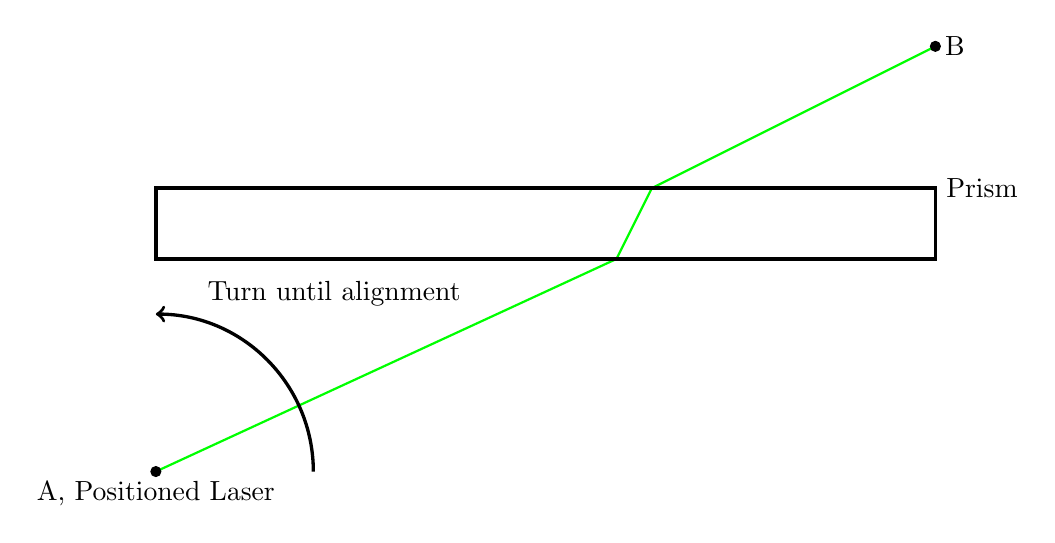
\begin{tikzpicture}[scale=0.9]
\draw[green, thick] (-2,0) -- (4.5,3);
\draw[green, thick] (4.5,3) -- (5,4);
\draw[green, thick] (5,4) -- (9,6);
\filldraw[black] (-2,0) circle (2pt) node[anchor=north,] {A,\ Positioned Laser};
\filldraw[black] (9,6) circle (2pt) node[anchor=west] {B};
\draw[very thick] (-2,3) rectangle (9,4) node[anchor=west]{Prism};
\draw[opacity=0]
(-2,3) coordinate (a) node[anchor=west]{}
(-2,0) coordinate (b) node[anchor=west]{}
(0,0) coordinate (c) node[anchor=west]{}
pic["Turn until alignment",draw=black, very thick, angle eccentricity=1.6, angle radius=2cm, opacity=1, ->]
{angle=c--b--a};
\end{tikzpicture}

\clearpage
\section*{Deriving an equation}
To achieve our solution to the problem we first derived an equation for the cost in terms of the the east. As we are able to assume the location of the forest, we assumed that it was the furthest north possible, so that there are two sections of the route, $a$ outside the forest and $b$ inside the forest. We can then state an equation for the cost, $C$, as:

\[ C = |a| + 2|b| \]

To calculate $|a|$ and $|b|$ we simply use Pythagoras' Theorem, however the distance east to where the route reaches the forest is unknown, so we let this distance be $x$ as shown.\\

%Diagram with east distance in X
\begin{tikzpicture}
\draw[gray, thick] (-2,0) -- (8,5);
\draw[gray, thick] (8,5) -- (9,6);
\filldraw[black] (-2,0) circle (2pt) node[anchor=north] {City A};
\filldraw[black] (9,6) circle (2pt) node[anchor=west] {City B};
\draw[very thick] (-2,6) rectangle (9,5) node[anchor=west]{forest};
\draw [opacity = 0]
(9,6) coordinate (b) node[anchor=west]{}
-- (8,5) coordinate (a) node[anchor=west]{}
-- (8,7) coordinate (c) node[anchor=west]{}
pic["$\theta_{2}$",draw=red,angle eccentricity=1.5,angle radius=0.5cm, opacity = 1] {angle=b--a--c};
\draw [opacity = 0]
(8,3) coordinate (b) node[anchor=west]{}
-- (8,5) coordinate (a) node[anchor=west]{}
-- (-2,0) coordinate (c) node[anchor=west]{}
pic["$\theta_{1}$",draw=red,angle eccentricity=1.2,angle radius=1cm, opacity = 1] {angle=c--a--b};
\draw[dashed] (8,3) -- (8,6.5);
\draw[<->] (8,6.5) -- (9,6.5);
\draw[<->] (-2,6.5) -- (8,6.5);
\draw[<->] (-3,6) -- (-3,5);
\draw[<->] (-3,5) -- (-3,0);
\draw (8.5,6.5) node[anchor=south]{$70-x$};
\draw (3,6.5) node[anchor=south]{$x$};
\draw (-3,5.5) node[anchor=east]{$7.5$};
\draw (-3,2.5) node[anchor=east]{$32.5$};
\draw (3,2) node[anchor=west]{$\mathbf{a}$};
\draw (8.4,5.3) node[anchor=west]{$\mathbf{b}$};
\end{tikzpicture}
Hence\\
$|a| = \sqrt{x^2+32.5^2}$\\
\\
$|b| = \sqrt{(70-x)^2+7.5^2}$,
\[\Rightarrow C=\sqrt{x^2+32.5^2}+2\cdot\sqrt{(70-x)^2+7.5^2}\]
\clearpage
We then differentiate this equation and let $\frac{dC}{dx} = 0$ to find the value of $x$ for the most cost-efficient route.\\
\\

\noindent $C=\sqrt{x^2+32.5^2}+2\cdot\sqrt{(70-x)^2+7.5^2}\\
\\
\\
Let\  a=\sqrt{x^2+32.5^2}\\
Let\  u=x^2+32.5^2\\
\\
\frac{da}{dx} = \frac{da}{du} \cdot \frac{du}{dx} = \frac{1}{2}\cdot(x^2+32.5^2)^{-\frac{1}{2}}\cdot2x\\
\\
\\
Let\ b=2\cdot\sqrt{(70-x)^2+7.5^2}=2\cdot\sqrt{x^2-140x+70^2+7.5^2}\\
Let\ v=(70-x)^2+7.5^2=x^2-140x+70^2+7.5^2\\
\\
\frac{db}{dx}=\frac{db}{dv}\cdot\frac{dv}{dx}=2\cdot\frac{1}{2}\cdot(x^2-140x+70^2+7.5^2)^{-\frac{1}{2}}\cdot(2x-140)
\\
\\
\\
\\
\frac{dC}{dx}=\frac{da}{dx}+\frac{db}{dx}\\
\\
=\frac{1}{2}\cdot(x^2+32.5^2)^{-\frac{1}{2}}\cdot2x + 2\cdot\frac{1}{2}\cdot(x^2-140x+70^2+7.5^2)^{-\frac{1}{2}}\cdot(2x-140)\\
\\
=\frac{x}{\sqrt{x^2+32.5^2}}+\frac{2x-140}{\sqrt{x^2-140x+70^2+7.5^2}}$\\
\\

\noindent And, where the cost is minimum,
\[\frac{x}{\sqrt{x^2+32.5^2}}+\frac{2x-140}{\sqrt{x^2-140x+70^2+7.5^2}}=0\]

\clearpage
\section*{Numerical solution}
As the equation is complex, and the graph of \[y=\frac{x}{\sqrt{x^2+32.5^2}}+\frac{2x-140}{\sqrt{x^2-140x+70^2+7.5^2}}\]
shows that there is a single solution:\\

%graph
\begin{figure}[ht]
    \centering
    \includegraphics[scale=0.08]{desmos-graph}
\end{figure}


We used a numerical method to find the solution to an appropriate degree of accuracy, by testing values for $1<x<70$ and observing the interval at which a sign change occurs. This is then repeated within that interval and so on, until we can determine that $x=66.23$ to 4.s.f. The Table of outputs is shown below where $f(x) = \frac{x}{\sqrt{x^2+32.5^2}}+\frac{2x-140}{\sqrt{x^2-140x+70^2+7.5^2}}$
\begin{figure}[ht!]
    \centering
    \includegraphics[scale=0.35]{TABLE.png}
    \captionsetup{labelformat=empty}
    \caption{Table of outputs}
\end{figure}

\clearpage
\section*{Calculation of Cost \& Route}

Using $x=66.23$ in the original equation for $C$, the cost of the route can be evaluated:\\
\\
\\
$C=\sqrt{x^2+32.5^2}+2\cdot\sqrt{(70-x)^2+7.5^2}\\
=\sqrt{66.23^2+32.5^2}+2\cdot\sqrt{(70-66.23)^2+7.5^2}\\
=90.56\ \mbox{to 4.s.f}$
\\
\\
This is lower than the cost of both tested cases going directly north through the forest and directly to city B in a straight line, which is evidence that the solution is valid.\\
The angles to the normal at each section of the route can also be determined:
\\
\\
$\tan{\theta_{1}} = \frac{66.23}{32.5}\\
\Rightarrow \theta_{1}=\arctan{\frac{66.23}{32.5}}=63.86^{\circ}\\
\\
\tan{\theta_{2}} = \frac{70-66.23}{7.5}\\
\Rightarrow \theta_{2}=\arctan{\frac{70-66.23}{7.5}}=26.69^{\circ}$
\\
\\
for the most cost-efficient route as shown in the figure below.
\\
\\
\\
%Diagram of most cost efficient route
\begin{tikzpicture}
\draw[gray, thick] (-2,0) -- (8,5);
\draw[gray, thick] (8,5) -- (9,6);
\filldraw[black] (-2,0) circle (2pt) node[anchor=north] {City A};
\filldraw[black] (9,6) circle (2pt) node[anchor=west] {City B};
\draw[very thick] (-2,6) rectangle (9,5) node[anchor=west]{forest};
\draw [opacity = 0]
(9,6) coordinate (b) node[anchor=west]{}
-- (8,5) coordinate (a) node[anchor=east]{}
-- (8,7) coordinate (c) node[anchor=west]{}
pic["$26.69^{\circ}$",draw=red,angle eccentricity=1.5,angle radius=1.1cm, opacity = 1] {angle=b--a--c};
\draw [opacity = 0]
(8,3) coordinate (b) node[anchor=west]{}
-- (8,5) coordinate (a) node[anchor=west]{}
-- (-2,0) coordinate (c) node[anchor=west]{}
pic["$63.86^{\circ}$",draw=red,angle eccentricity=1.5,angle radius=1.1cm, opacity = 1] {angle=c--a--b};
\draw[dashed] (8,3) -- (8,7);
\end{tikzpicture}
\clearpage
\section*{Evaluation \& Conclusion}

This model achieves a reasonably accurate solution to the problem presented, however there are some alterations that may refine the model to increase accuracy or applicability to the real-life scenario.\\
\indent The first to consider is the use of a numerical method to find $x$ for the minimum cost. This is not an exact solution and it may improve the accuracy find and use an exact solution algebraically. Secondly, the assumption that the north-south location of the forest is irrelevant - The assumption was made by observation of the scenario, and so it may be necessary to devise a more rigorous proof. It has also been assumed that the roads constructed are straight, the roads are flat, i.e. built on flat terrain, and that they have no width. More information may be required to refine the model, such as details on the topography of the land so the road can be considered in three dimensions. If the land were not perfectly flat as assumed, the road would have greater length and therefore greater cost, and so may not be the most cost-efficient route in reality.\\
\indent It has been shown that it is not the most cost-efficient route to travel directly north through the forest as questioned in the problem statement. It has otherwise been determined that the most cost-efficient route is to travel at $63.86^{\circ}$ to the normal outside the forest and $26.69^{\circ}$ to the normal inside of the forest, for a minimum cost of $90.56$.



\clearpage
\printbibliography


\end{document}
